\begin{figure}[ht] 
 	\centering 
 	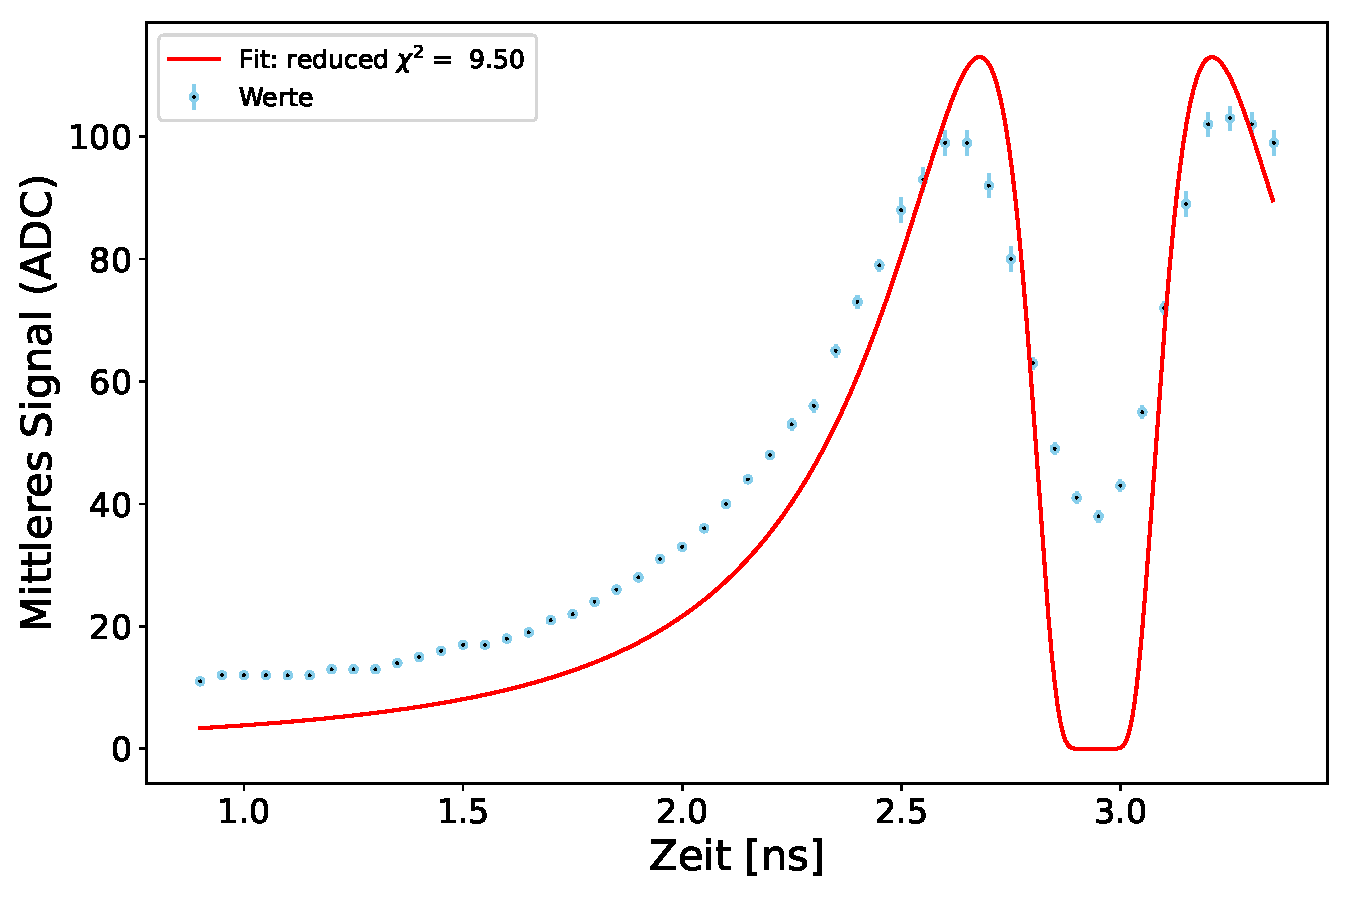
\includegraphics[width= 0.65 \textwidth]{Fits/Amps_B06A_Fit.pdf} 
	\caption{Amps_B06A, Fit} 
 	\label{fig:Amps_B06A, Fit} 
\end{figure}
 \\ 
\begin{table}[ht] 
\centering 
\caption{Amps_B025A, Fit Parameter Tabelle} 
\label{tab:my-table}
\begin{tabular}{|l|c|}
\hline
Parameter Name	&	Wert \\ \hline
g	&	 8.413 \pm  0.579\\ \hline
amp	&	 0.482 \pm  0.0384\\ \hline
\end{tabular} 
\end{table}